% chapters/background.tex
\chapter{Background}
\label{ch:background}

\section{Object Detection with YOLO}
\label{sec:yolo}

% General YOLO introduction
YOLO (You Only Look Once) is a family of real-time object detection models first introduced by \citet{redmon2016yolo} and now maintained by Ultralytics \citep{yolov8}. Unlike two-stage detectors that first propose regions and then classify them, YOLO performs detection in a single forward pass, which is what makes it fast enough for our use case. We evaluated three successive generations of nano-sized YOLO models.

\subsection{YOLO11}
\label{subsec:yolo11}

% YOLO11 overview
YOLO11 was released in 2024 by Ultralytics \citep{yolo11} and is the architecture currently deployed on the UBM race car. It introduces C3k2 backbone blocks, a Spatial Pyramid Pooling Fast (SPPF) layer, and C2PSA attention modules. The nano variant has 2.59M parameters and 6.4 GFLOPs. This is our baseline: every other model in this report is measured against it.

\subsection{YOLO12}
\label{subsec:yolo12}

% YOLO12 overview
YOLO12, published in January 2025 by \citet{yolo12}, replaces the CSP backbone with R-ELAN (Residual Efficient Layer Aggregation Network) and introduces an area-attention mechanism that captures global context without the quadratic cost of standard self-attention. The nano variant sits at 2.56M parameters and 6.3 GFLOPs, marginally smaller than YOLO11n. 
\subsection{YOLO26}
\label{subsec:yolo26}

% YOLO26 overview
YOLO26 is the most recent release from Ultralytics at the time of writing \citep{yolo26}. Its nano variant is the smallest of the three we evaluated: 2.51M parameters and 5.8 GFLOPs. It also eliminates the non-maximum suppression (NMS) post-processing step, further reducing latency.

\section{Transfer Learning and Catastrophic Forgetting}
\label{sec:transfer}

% Transfer learning concepts
Transfer learning is the practice of pre-training a model on a large dataset and then fine-tuning it on a smaller, task-specific one \citep{cone_detector, fsoco12}. The main risk is catastrophic forgetting \citep{catastrophic_forgetting}: if the learning rate is too high during fine-tuning, the model overwrites the useful features it learned during pre-training. Standard mitigation strategies include freezing early layers, using a low learning rate, and warming up gradually. We encountered this problem during our two-stage training and document the diagnosis and fix in \cref{sec:two_stage,app:optimizer_bug}.

\section{Model Optimization for Edge Deployment}
\label{sec:optimization}

% ONNX and TensorRT overview
The models are trained in PyTorch but deployed through a multi-stage optimization pipeline. First, the trained weights are exported to ONNX (Open Neural Network Exchange) \citep{onnx}, a hardware-agnostic intermediate representation. Then, NVIDIA TensorRT \citep{tensorrt} compiles the ONNX graph into an optimized engine for the target GPU. TensorRT applies several automatic optimizations: kernel fusion combines sequences of operations (e.g.\ Conv$+$BatchNorm$+$ReLU) into a single GPU kernel to reduce memory bandwidth and kernel launch overhead, and precision reduction converts FP32 weights to FP16 or INT8 to exploit the GPU's dedicated Tensor Cores. INT8 quantization requires a calibration dataset of 500--1{,}000 representative images to determine the optimal scaling factors, and typically incurs a 2--3\% \mAPfifty{} drop compared to FP16.

One practical constraint is that TensorRT selects kernels and memory layouts optimized for the specific GPU it builds on. While GPUs within the same generation (e.g.\ RTX 4080 Super and RTX 4060, both Ada Lovelace) share compute capability 8.9, an engine built on one cannot run on the other, since only building on the target hardware ensures optimal kernel selection. We therefore built the final engine directly on the race car's RTX 4060.

\section{Formula Student Driverless Perception}
\label{sec:fsd}

% Perception pipeline overview
The perception pipeline, as designed by \citet{fusa2025}, is built around a ZED 2i stereo camera \citep{zed2i} operating at 1280$\times$720 resolution and 30~fps but targeting 60~fps in the future. The YOLO detector runs on each frame to produce 2D bounding boxes for five cone classes defined by the FSAE Driverless rules \citep{fsae_rules}: small blue cones mark the left track border, small yellow cones mark the right border, small orange cones delineate entry and exit lanes, and large orange cones are placed before and after start, finish, and timekeeping lines. A fifth class, ``unknown,'' is used for ambiguous or occluded cones that cannot be confidently classified. These detections are then matched across the stereo pair and triangulated to produce 3D positions relative to the car. Any excess time taken by detection directly reduces the budget available for planning and control downstream.

\section{Related Work}
\label{sec:related}

% Related work
The FSOCO (Formula Student Objects in Context) dataset \citep{fsoco} is a community-maintained benchmark for cone detection, contributed by multiple Formula Student teams. It provides a shared evaluation standard, though the images come from a variety of cameras and conditions that may not match any single team's deployment setup. Most teams in the Driverless competition use some variant of YOLO, trained on FSOCO or private datasets, and evaluate using the standard COCO metrics \citep{coco}: \mAPfifty{} (intersection-over-union threshold of 0.5) and \mAPfiftyfive{} (averaged over thresholds from 0.5 to 0.95). The prior work at UBM is documented in the thesis by \citet{fusa2025}, which established the YOLO11n baseline and the stereo matching pipeline we build upon.

\begin{figure}[ht]
\centering
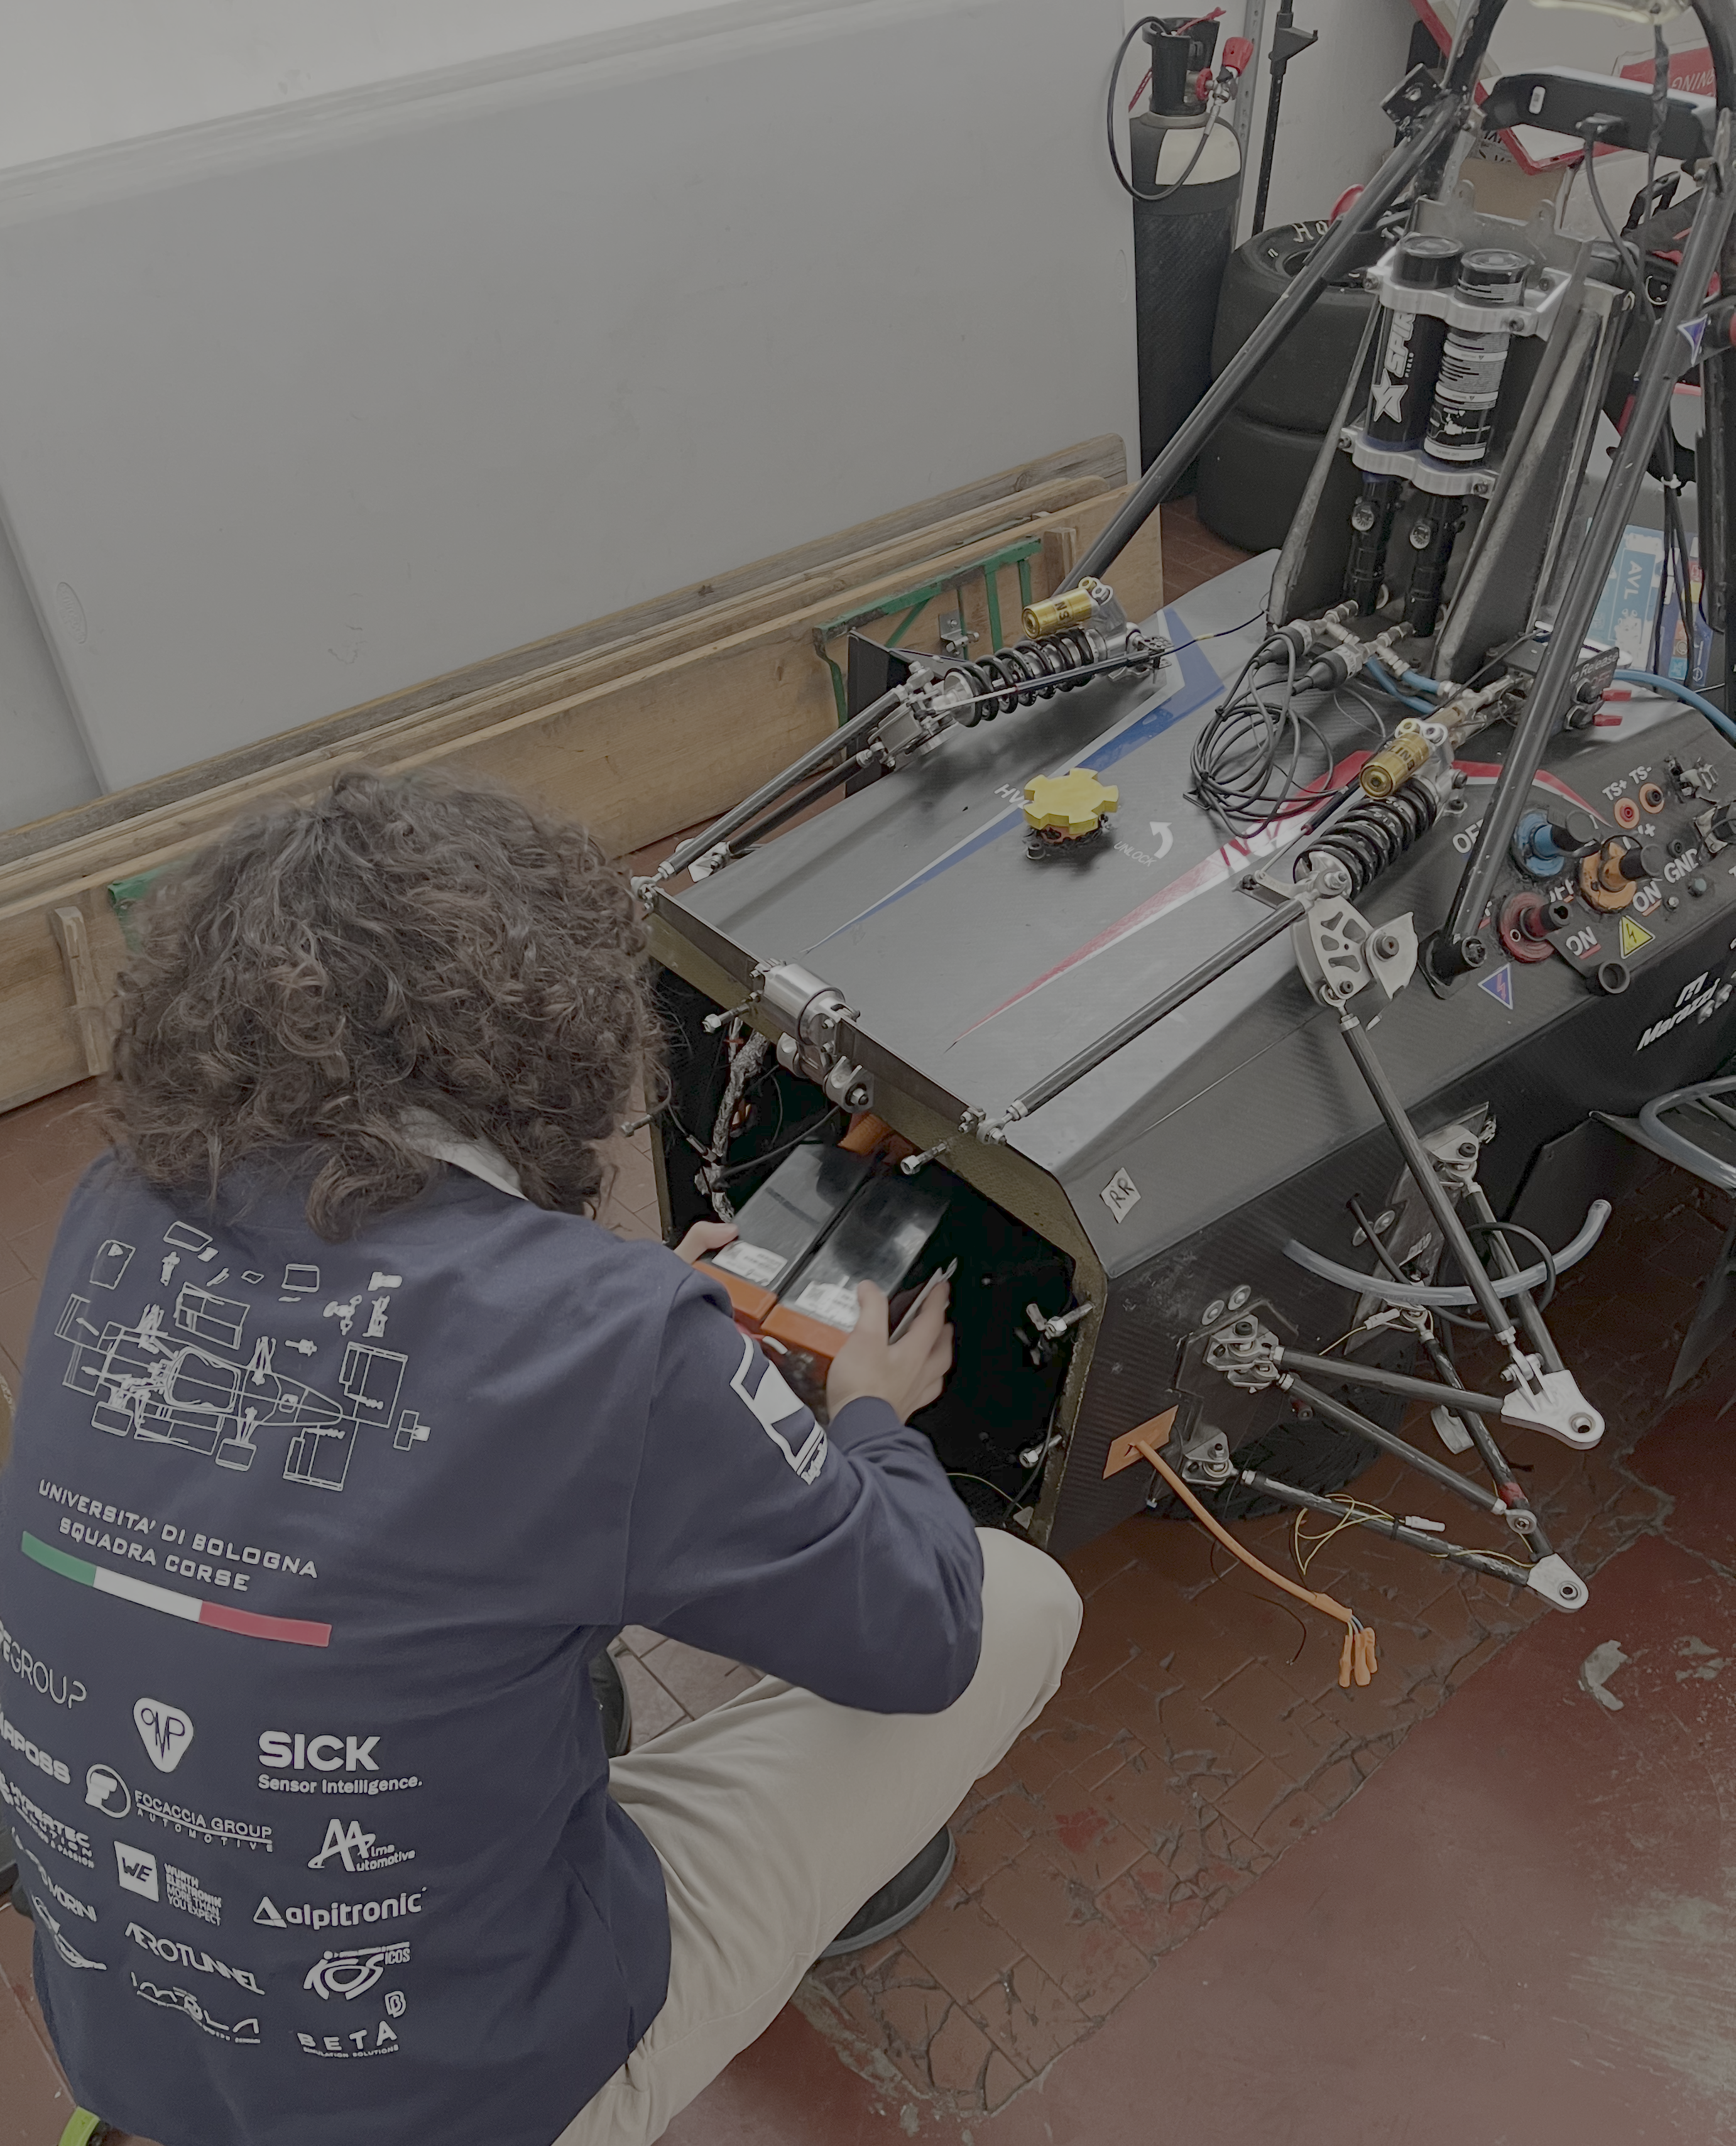
\includegraphics[width=0.5\textwidth]{racecar.jpg}
\caption{The rear of the racecar inside the UBM Workshop while removing the 12v battery which powers the computers.}
\label{fig:racecar}
\end{figure}